\documentclass{article}
\usepackage{xcolor}
\usepackage{titleps}
\usepackage[letterpaper, margin=0.95in]{geometry}
\usepackage{url}
\usepackage{amsmath}
\usepackage{amssymb}
\usepackage{wrapfig}
\usepackage{float}
\usepackage{mathtools}
\usepackage{enumitem}
\usepackage{tabu}
\usepackage{parskip}
\usepackage{natbib}
\usepackage{listings}

\usepackage{hyperref}
\usepackage[color=red]{todonotes}
\usepackage{forest}
\definecolor{light-yellow}{HTML}{FFE5CC}

\newpagestyle{ruled}
{\sethead{CMU 16-831}{Intro to Robot Learning}{Spring 2024}\headrule
  \setfoot{}{}{}}
\pagestyle{ruled}

\renewcommand\makeheadrule{\color{black}\rule[-.75\baselineskip]{\linewidth}{0.4pt}}
\renewcommand*\footnoterule{}

\begin{document}
\lstset{basicstyle = \ttfamily,columns=fullflexible,
backgroundcolor = \color{light-yellow}
}

\begin{centering}
    {\Large Assignment 1: Imitation Learning} \\
    \vspace{.25cm}
    \textbf{Andrew ID:} \texttt{yxiu2} \\
    \textbf{Collaborators:} \texttt{yxiu2}\\ 
\end{centering}

\vspace{.5cm}

\section{Behavioral Cloning}
\subsection{Part 2}

\begin{table}[h]
\centering
\begin{tabular}{|l|c|r|} % l = left, c = center, r = right
\hline
Environment & Mean & Standard Deviation \\
\hline
Ant-v2 & 4713.65 & 12.19 \\
Humanoid-v2 & 10344.52 & 20.98 \\
Walker2d-v2 & 5566.85 & 9.24 \\
Hopper-v2  & 3772.67 & 1.95 \\
HalfCheetah-v2 & 4205.78 & 83.04 \\
\hline
\end{tabular}
\caption{Mean and Standard deviation of return over five trajectories of the expert data.}
\label{tab:part1}
\end{table}

\subsection{Part 3}

\begin{table}[h]
\centering
\begin{tabular}{|l|c|c|c|r|} % l = left, c = center, r = right
\hline
Environment & Eval\_AverageReturn & Eval\_StdReturn & Initial\_DataCollection\_AverageReturn & Performances\\
\hline
Ant-v2 & 1512.86 & 1049.34 & 4713.65 & 32.09\% \\
Humanoid-v2 & 267.94 & 69.69 &10344.51 & 2.59\%\\
% Walker2d-v2 & 5566.85 & 9.24 &4713.65 &\\
% Hopper-v2  & 3772.67 & 1.95 &4713.65 &\\
% HalfCheetah-v2 & 4205.78 & 83.04 &4713.65 &\\
\hline
\end{tabular}
\caption{Mean, Standard deviation and perfomances over trajectories of the expert data in environment Ant and Humanoid. The behavioral cloning agent in the Ant environment could achieve 32.09\% of the performance of the expert, while and in the Humanoid environment, the performance only achieves 2.59\%. Both evaluations are conducted on five rollouts, where the eval\_batch\_size is 5000 and ep\_len is 1000. For a fair comparison, both training and evaluations are run with the same hyperparameters such as network size = 64, number of training iterations = 1000, and n layers = 2.}
\label{tab:part2}
\end{table}

\subsection{Part 4}

\begin{figure}[ht]
\centering
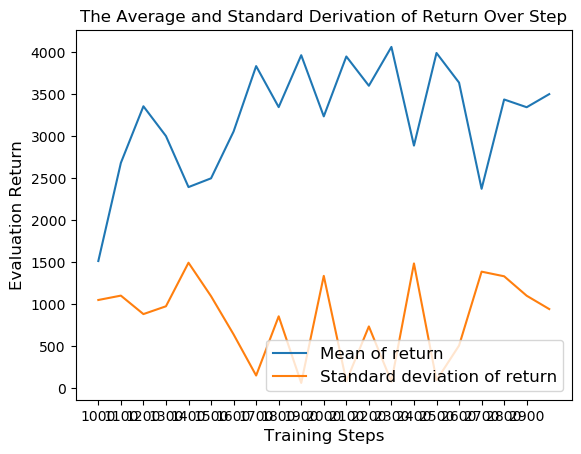
\includegraphics[width=0.4\linewidth]{part_3.png}
\caption{The Figure shows Ant-v2 BC agent's performances with different training steps from 1000 to 3000. The hyperparameters are set with same network size 64 and n layer = 2, the eval\_batch\_size is 5000 and ep\_len is 1000. The reason of modifying training steps is, we believe the network would have better performance as the network are trained with more steps to fit the data. The empirical performance seems to increase after 1000 steps as the average return goes higher, but still with large oscillations.}
\label{fig:image1}
\end{figure}

\clearpage


\section{DAgger}
\subsection{Part 2}

\begin{figure}[ht]
\centering
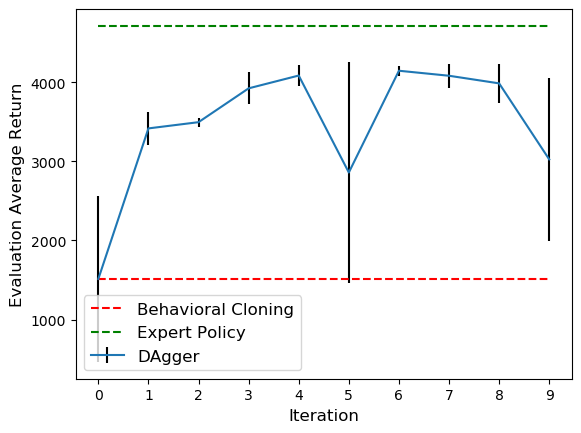
\includegraphics[width=0.5\linewidth]{Q2_2_Ant.png}
\caption{The Figure shows Ant-v2 agent's performance for DAgger, BC, and expert policy in Ant environment. The hyperparameters are set with same network size 64 and n layer = 2, training\_steps = 1000, the eval\_batch\_size is 5000 and ep\_len is 1000, which collects five rollouts.}
\label{fig:image2}
\end{figure}

\begin{figure}[ht]
\centering
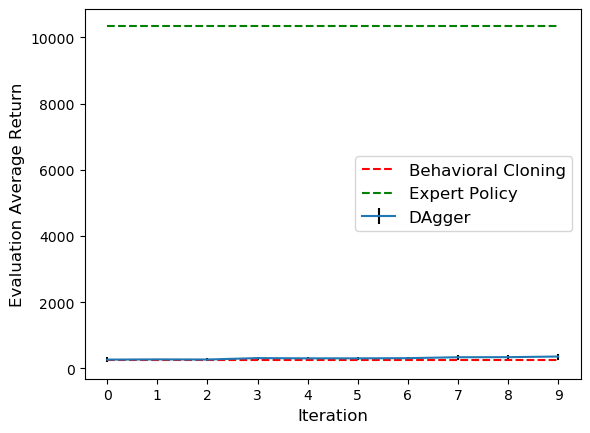
\includegraphics[width=0.5\linewidth]{Q2_2_Humanoid.png}
\caption{The Figure shows Humanoid-v2 agent's performance for DAgger, BC, and expert policy in Humanoid environment. The hyperparameters are set with same network size 64 and n layer = 2, the eval\_batch\_size is 5000 and ep\_len is 1000, which collects five rollouts.}
\label{fig:image3}
\end{figure}

\end{document}